\section{Background}\label{sec:background}
%For CPSs different models can be coupled together into multi-models using co-simulation \cite{Gomes&18,Thule&19}. In the INTO-CPS context this have been established using the Functional Mockup Interface (FMI) standard~\cite{FMIStandard2.0}\footnote{\url{http://fmi-standard.org/}}, supports co-simulation of models packaged as Functional Mock-up Units (FMUs), each of which is treated as a `black box', supporting the separation of Intellectual Property (IP).

It is important to make a distinction between what the FMI standard defines and the information required to form a valid co-simulation scenario as illustrated on Figure~\ref{fig:connection}. 
The standard is solely concerned with specifying the interface of an individual FMU.
A co-simulation scenario describes what instances of FMUs exist, how they are connected, their parameters and their experimental frame~\cite{Gomes&18}. In order to provide the reader with sufficient background about the existing technologies Section~\ref{sec:sysml} briefly introduces the existing SysML diagrams to describe the composition of FMUs, Section~\ref{sec:adaptation} provides a brief introduction to separate existing work on semantic adaptation including hierarchical compositions and Section~\ref{sec:SSP} provides a brief introduction to the new SSP standard. 

\subsection{Existing SysML Connection Diagram}\label{sec:sysml}

A SysML Internal Block Diagram in the context of INTO-CPS is referred to as a \emph{Connection Diagram}.
It is used to define the composition and connectivity of several FMUs. The connection diagram contains instances of FMUs (SysML Block instances) which are connected together by means of connectors to the input/output ports of the FMU instances. The connection diagram also enables association of existing FMUs to the block instances for a co-simulation.

\begin{figure}[bt]
\centering
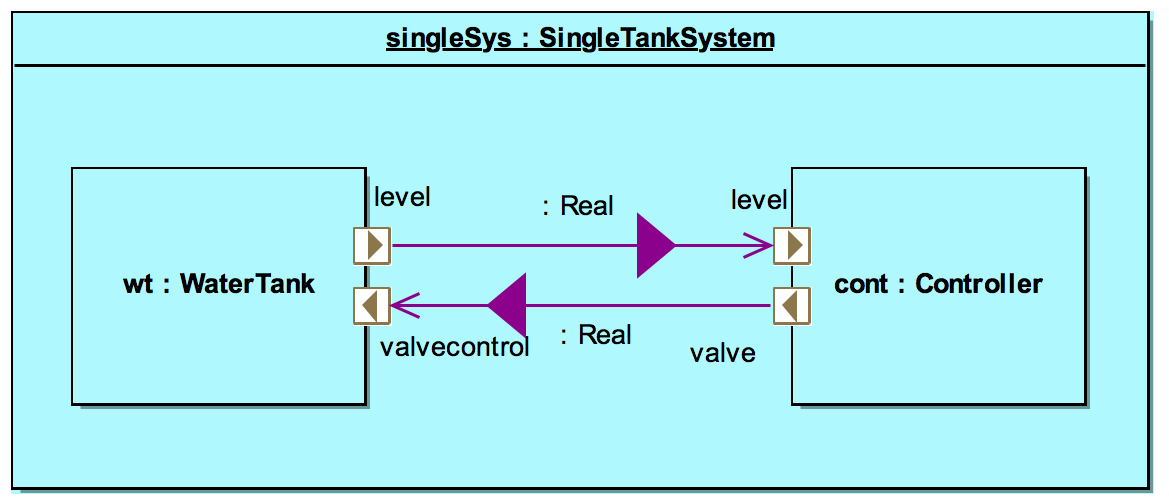
\includegraphics[width=.8\columnwidth]{Images/sysml_cd}
\caption{Connection diagram for the WaterTank example to connect FMUs.}
\label{fig:connection}
\end{figure}


Using a general-purpose modeling language such as SysML for defining simulation scenarios, comes with an inherent challenge.
The lack of simulation specific concepts in the language makes expression of these more cumbersome and error prone.
First, it is required that the users memorise the exact way these concepts must be expressed in SysML.
Secondly, it limits the assistance the tool can provide the user, due to its limited understanding of domain specific concepts.  
These issues are amplified by the fact that errors are only detected when the SysML model is imported in the tool.

In the DSE diagrams inside the SysML profile the exploration capabilities makes use of parameters for the different FMUs, so this is also important for the work we describe here.


\subsection{Semantic Adaptations}\label{sec:adaptation}

While the FMI standard defines a common format for exchanging FMUs it does not guarantee the absence of so called \emph{interaction mismatches} when these are composed \cite{Gomes&18a}.
The goal of semantic adaptations~(SA), is to allow these mismatches to be corrected without the need to involve the original author of the FMU.

A concrete example where this would be if \emph{valve} input of the \emph{WaterTank} accepted a bool instead of a real.
In this case it would not be possible to connect the \emph{valvecontrol} and \emph{valve} ports.
A SA could be used to apply a threshold to the \emph{valve} output in order to convert it into a bool, as seen in figure~\ref{fig:watertank_SA}.

\begin{figure}[bt]
\centering
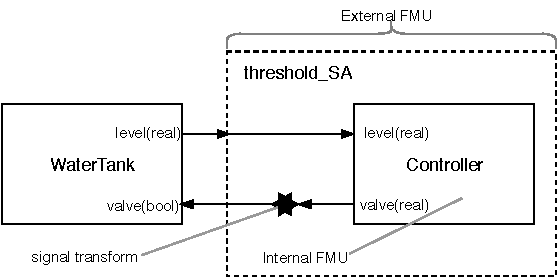
\includegraphics[width=0.8\columnwidth]{Images/watertank_SA.pdf}
\caption{Example of how semantic adaptation may be applied to correct signal data mismatch.}
\label{fig:watertank_SA}
\end{figure}


Conceptually, a SA can be thought of as an \emph{external} FMU, which wraps around one or more \emph{internal} FMUs. The external FMU is responsible for managing the execution of the internal FMUs. In the previous example the external FMU would simply pass all signals directly, except for the \emph{valve}, which would be thresholded before being written to the \emph{valve} output of the external FMU.  
The approach grants a great deal of flexibility, allowing a large number of adaptations to be implemented. In addition, it allows these to be applied in a hierarchical manner, e.g. "on top of" each other.

As described in Section~\ref{sec:intro} the SysML CPS profile does not yet support semantic adaptations \cite{Gomes&18a}. In general such semantics adaptations are currently established by a separate Domain Specific Language (DSL). This is introduced in order to perform different kinds of adaptations to existing FMUs that enable their behaviour to be adjusted in different ways. However, the DSL from \cite{Gomes&18a} also enables support for hierarchical co-simulations. A different approach for hierarchical co-simulations has been introduced in \cite{Thule&19}. 


%This work seeks to find a graphical representation that is easy to apply while remaining sufficiently %expressive.


%Graphically most of these can be represented as different kinds of annotations.

%There are several important differences in concepts and notation used within INTO-CPS toolchain and the SSP.
%A superficial understanding these are essential to following the discussion and design choices of the editor.
%While being designed as a complementary standard for FMI; SSP is agnostic towards the implementation details of a simulation unit.
%To emphasize this its uses the word \emph{component} instead of FMU.
%A crucial detail is that a component may itself be a SSP package \cite[p.53]{SSP19}.
%If this is the case it is referred to as a \emph{subsystem}.
%Another difference is that one SSP package may be contain several so called \emph{systems}.
%In the context of the editor, a system is equivalent to a multi model.


\subsection{System Structure And Parametrisation}\label{sec:SSP}

The central goal of the INTO-CPS Application is to enable the composition and co-simulation of a system consisting of one or more FMUs. 
The use of the FMI standard enables exchange at the level of the individual FMUs.
However, it does not describe an exchange format for composing and parametrising a simulation scenario consisting of multiple FMUs.
Due to the lack of an established standard, the INTO-CPS Application uses its own ad-hoc format referred to as the \emph{multi-model} format.

Recently a new companion standard to FMI was published: the \emph{System Structure and Parameterization} (SSP) standard~\cite{SSP19}\footnote{\url{https://ssp-standard.org/}}.
The standard uses a zip-based packaging format similar to FMI, where multiple artefacts are bundled into a single package referred to as a \emph{SSP package} -- each representing a ready to simulate system.
An obvious benefit of adopting this standard is exchangeability of complete systems between tools. Currently only a few such as OpenModelica and \emph{FMPy}\footnote{\url{https://github.com/CATIA-Systems/FMPy}}, however given its close relation to FMI, it seems likely that more tools will adopt it. 
An example of what the running example may look like when bundled as a package is seen on Figure~\ref{fig:ssp_structure}.

The standard covers the functionality present in the existing format, but also adds several capabilities which are useful for the INTO-CPS Application.
Additionally, there are also some important semantic differences between the existing format and SSP.
Ultimately, some of these influence the interaction in the GUI editor, as such the most relevant differences are highlighted below.

\begin{description}
\item[Components and Hierarchy:]
While the standard is closely aligned with the FMI it is not limited to describing systems purely consisting of FMUs.
Instead the standard establishes the concept of a \emph{component} -- an atomic block of the system, which is backed by some underlying implementation.
For example, a component may reference a FMU as its implementation.
A component may itself be a SSP package, which in this context, is referred to as a \emph{sub-system}. 
The latter enables the creation of hierarchies of components.


\item[Parameterization:]
There is an important difference between how parameters are treated in a multi-model and by SSP.
In the former all parameters are defined inline, there is no mechanism to reference a ``shared'' parameter from multiple components.
SSP on the other hand provides the \emph{parameter sets} and \emph{parameter mappings} concepts which makes it possible to declare a set of parameters and then bind these to the concrete components\footnote{Inside the SSP standard these are referred to as System Structure Parameter Values and System Structure Parameter Mappings.}.

\item[Extensibility:]
Similar to FMI the standard is largely based on XML and is designed to be extensible through three types of extension mechanisms: Annotations, extra files and MIME type-based format dispatch.
This allows for the creation of new extensions to the standard referred to as \emph{layered standards}.
A potential use case of this is to extend the standard with support for semantic adaptations.
\end{description}

%Annotations can be applied to several XML elements, for example a component. The annotation may contain arbitrary XML data.


%\begin{figure}[bt]
%\centering
%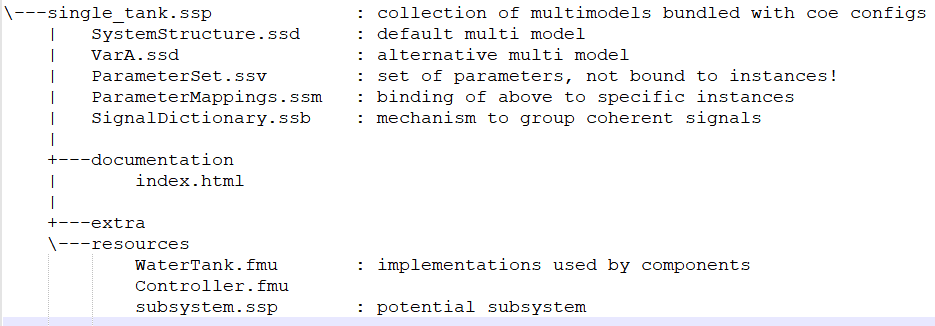
\includegraphics[width=\columnwidth]{Images/ssp_structure.png}
%\caption{}
%\label{fig:ssp_structure}
%\end{figure}



\begin{figure}[bt]
\centering

\begin{Verbatim}[tabsize=4,fontsize=\small,samepage=true,frame=single]
\---single_tank.ssp         : collection of multi models
    | SystemStructure.ssd   : default multi model
    | VarA.ssd              : alternative multi model
    | ParameterSet.ssv      : set of parameters
    | ParameterMappings.ssm : binding params to instances
    | SignalDictionary.ssb  : mechanism to group signals
    |
    +---documentation
    | index.html
    |
    +---extra               : extra files extension mechanism
    |
    \---resources           : implementations of components
      WaterTank.fmu
      Controller.fmu	
      subsystem.ssp         : potential subsystem
\end{Verbatim}

\caption{Example of the file structure of the running example stored as a SSP package. 
The comments on the side describe the role of the file. }
\label{fig:ssp_structure}
\end{figure}
%\begin{figure}[bt]
\centering
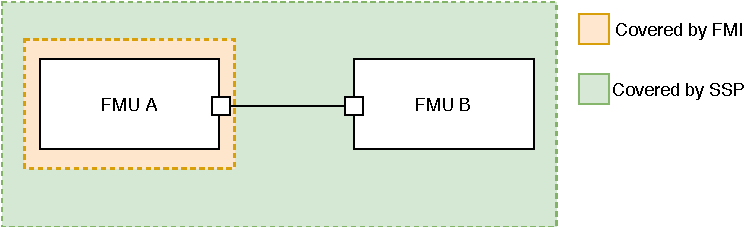
\includegraphics[width=0.8\columnwidth]{Images/fmi_vs_ssp.pdf}
\caption{Graphical depiction of domains that the FMI and SSP standards covers.
FMI describes the interface of the individual blocks. SSP defines the instances and connectivity of the FMUs}
\label{fig:fmi_vs_ssp}
\end{figure}

%A more in-depth discussion of the difference and migrations between the current and new format can be found in section~\ref{ssec:mm_vs_ssp}.


%However, when the application was initially developed no standard existed which describe how the individual FMUs %may be composed and parametrized.
%A graphical depiction of the domains covered by FMI and SSP can be seen in figure~\ref{fig:fmi_vs_ssp}.
%Adopting the new standard has clear benefits such as improving exchangeability between tools, being more %expressive and extensible than the current format.

%It is the a clear ambition of the developers of the INTO-CPS tool-chain to adopt SSP as the preferred format for %describing co-simulation scenarios.
%As such the rest of the paper assumes that the capabilities present in SSP is available for the graphical editor.
















